     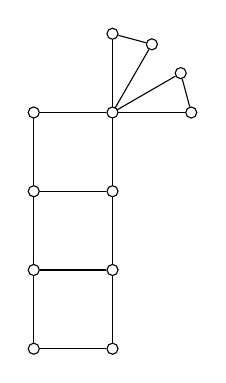
\begin{tikzpicture}

                \tikzstyle{vertex}  = [circle, minimum width=4pt, draw, inner sep=0pt, fill=white]
                \begin{scope}[shift={(1,3)}]

                \newdimen\R
                \R=1cm
                        \foreach \x in {0, 30, 60, 90}
                       {
                        \node [vertex](w\x) at (\x:\R) {};
                        \draw (0,0) -- (w\x);
                       }

                        \draw (w0) -- (w30);
                        \draw (w60) -- (w90);
                \end{scope}

                \foreach \x in {0, 1,...,3}
                {
                        \node [vertex](v\x) at (0, \x) {};
                        \node [vertex](u\x) at (1, \x) {};
                        \ifnum \x<3
                                \draw (v\x) -- ++(0,1);
                                \draw (u\x) -- ++(0,1);
                        \fi

                        \draw (u\x) -- (v\x);

                }

        \end{tikzpicture}


